%ब 

\section{Update} \label{s:results-update}
The \texttt{update} operation triggers  referential integrity validations
whenever entities of \texttt{Student},  \texttt{Course} and \texttt{Enrolment}
are updated with new values. Notice that the \texttt{Update} operation is
performed  on the primary keys of \texttt{Student} and \texttt{Course} entities,
 and on the foreign keys (\texttt{CourseId}) of \texttt{Enrolment}.
Figure~\ref{fres:Update} presents the results of the \texttt{update} operation
on each entity for all the solutions.
Figures~\ref{fres:Update-responsetime} and~\ref{fres:Update-throughput} present
the average response time and throughput of \texttt{update} on each entity in
all the solutions.

	\begin{figure}[H] 
		\subfigure[Response time for Update operation]
		{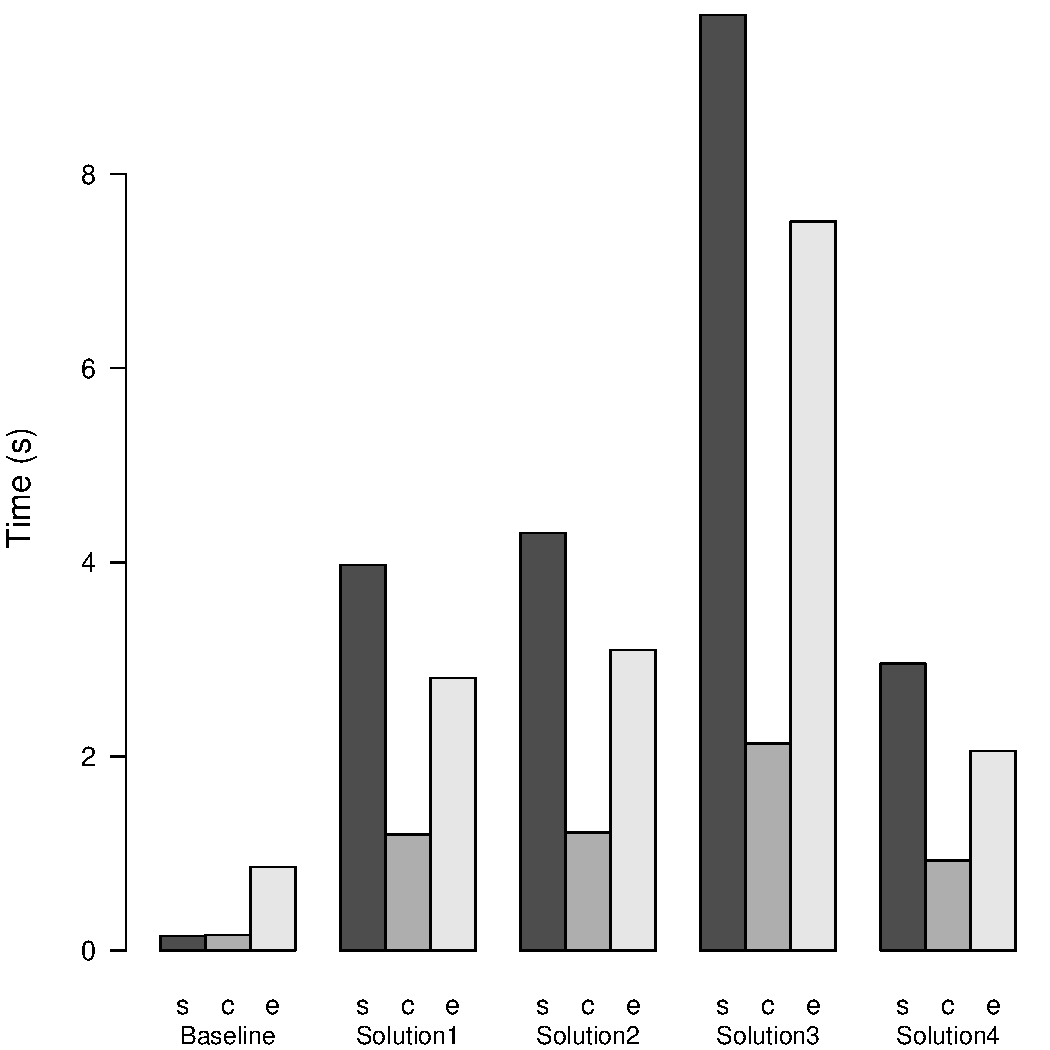
\includegraphics[width=\Width]{figure/result/barplot-update-rt.pdf}\label{fres:Update-responsetime}}
		\subfigure[Throughput for Update operation]
		{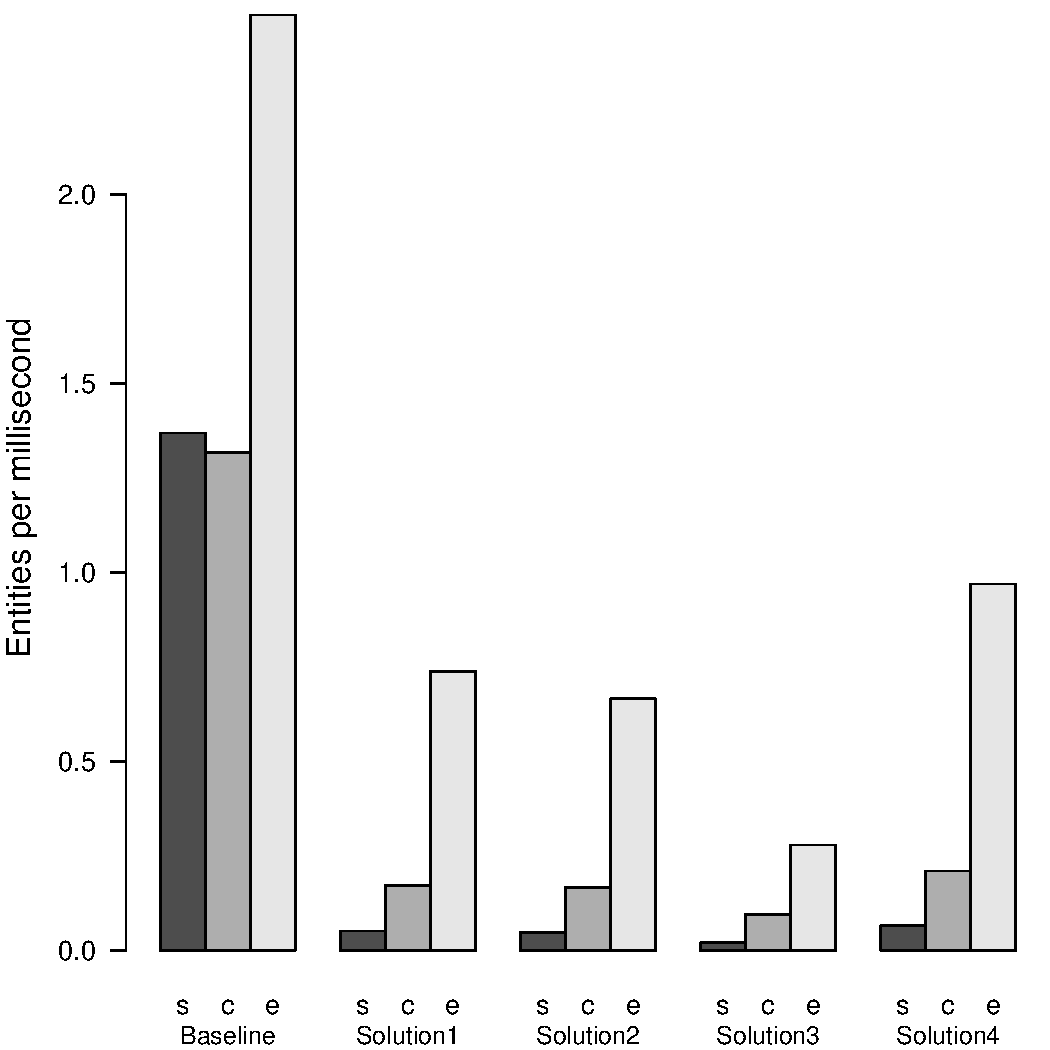
\includegraphics[width=\Width]{figure/result/barplot-update-tp.pdf}\label{fres:Update-throughput}}
		\caption{Performance of Solutions in Update}\label{fres:Update}
	\end{figure}
 
It can be seen from the results that the \texttt{update} operation on
\texttt{Enrolment} is  faster than \texttt{update} on a \texttt{Student} or
\texttt{Course} in all the solutions. 
The \texttt{update} operation  on a \texttt{Student} entity takes the most time
in all the solutions. 
The \texttt{update} operation on a \texttt{Course} entity always takes more time
than \texttt{update} on \texttt{Enrolment} but it is faster than updating
\texttt{Student} entities. The differences in  performance of 
\texttt{update} on the  entities is because of the referential integrity
rules that are applied during validation. 


Updating \texttt{Enrolment} is faster since before inserting the new values,  it
only  involves  identifying relevant \ac{FK} constraints in the metadata and 
accessing the parent column families \texttt{Student} and \texttt{Course} to
ensure that the new foreign key values exist.  Moreover,  \texttt{update} in
\texttt{Enrolment} involves changing the foreign key attributes and not the
primary key column. 

Updating \texttt{Student} is slower since the primary key is changed and it is a
cascaded operation that updates \texttt{Enrolment}.  After accessing the
relevant \ac{FK} constraints,  the child dependencies are retrieved from
\texttt{Enrolment} and updated with the new value for the \texttt{StudentId}.
This means that an \texttt{update} accesses the metadata as well as the child
column family and performs \texttt{insert} in \texttt{Student} and the child
column family \texttt{Enrolment} with the new values.  This operation also
involves performing a \texttt{delete} to remove the old primary key value in
\texttt{Student}.


Updating \texttt{Course} takes less time than \texttt{update} on
\texttt{Student} because it is not a cascaded operation as the
\texttt{DeleteRule} for \texttt{Course} entities is \texttt{NoDelete}\footnote{Notice that for the
  sake of simplicity, this rule is also used for update operations.} and
\texttt{Enrolment} contains its child dependencies.  Thus,  exceptions are
raised each time an \texttt{update} is performed on \texttt{Course} entities, 
which means that the response time includes measuring the time for validation as
well as raising exceptions.  But this is slower than \texttt{update} on
\texttt{Enrolment} because it involves accessing the \texttt{Enrolment} column
family to identify existing child dependencies.  Since these child dependencies
exist when the experiments are run,  the exceptions are raised each time.

% The time involved for an \texttt{update} on a \texttt{Course} entity is  more as
% seen in Figures~\ref{fres:Update} and~\ref{fres:update-course}.  In this
% operation the relevant \texttt{FK} constraints and child dependencies of the
% \texttt{Course} entity are identified and its  relevant \texttt{DeleteRule}
% is also determined. 
% Since the \texttt{DeleteRule} for \texttt{Course} entities is \texttt{NoDelete}
% an exception is raised.  Moreover,  \texttt{Enrolment} column family is accessed
% to identify existing child dependencies.  These additional operations and the
% exceptions raised make \texttt{update} on \texttt{Course} consume more time to
% complete. 
% 
% The results in Figures~\ref{fres:Update} and~\ref{fres:update-user} show that
% updating a \texttt{Student} entity takes the most time in all the solutions. 
% The relevant \ac{FK} constraints are accessed for this entity and
% its child dependencies are identified from \texttt{Enrolment},  which is similar
% to \texttt{update} on \texttt{course} entities.  However,  update on a
% \texttt{Student} entity is cascaded and involves updating all the child
% dependencies in \texttt{Enrolment} column family.  This means that an
% \texttt{update} causes writes not only in \texttt{Student} but also in the child
% column family \texttt{Enrolment}.  
Note that \texttt{update} on \texttt{Student} entities causes values to be
updated in two column families,  while on \texttt{Enrolment} values are
updated in only one column family and on \texttt{Course} no values are updated.  


Further details of the performance of each solution when the \texttt{update}
operation is executed on each entity is presented in
Figures~\ref{fres:update-response-time} and~\ref{fres:update-throughput}.
These results show that Solution~4 is the fastest amongst all the solutions, 
while Solution~3 is the slowest.
Solutions~1 and 2 perform almost similarly although the additional search for
the top row in Solution~2 makes it just slightly slower than Solution~1.
Note that in Solution~3 the \texttt{Metadata} column family is accessed multiple
times in each validation making it the slowest.  Multiple accesses are needed in
order to first retrieve the relevant \ac{FK} constraints and then to retrieve
information about the child or parent entities.  Although Solution~4 stores
metadata separately like Solution~3,  it caches and re-uses
% the \texttt{Metadata} column family and reuses the cache to avoid such multiple
% accesses to the column family.  
the list of constraints and avoids connecting to the external cluster to access
the \texttt{Metadata} column family each time  operations are invoked on entities.

When compared to the baseline,  the \texttt{update} operation on all the entities
take considerably more time in all the solutions because of their different
metadata storage designs.  The validations and metadata access for parent
entities make Solutions~1 and 2  almost more than 26 times slower than baseline. 
Solution~3 is almost 60 times slower than baseline while Solution~4 is only 20
times slower than the baseline  in such updates.  

However,  updates on child entities
make  Solution~1 and 2  more than 3 times slower than the baseline.  Solution~3
is nearly 8 times slower while 
Solution~4 is only 2 times slower than the baseline in such updates. 

\begin{landscape}
		\begin{figure}
		\centering
		\newcommand{\W}{.4\textwidth}
			\subfigure[Update on Student]
			{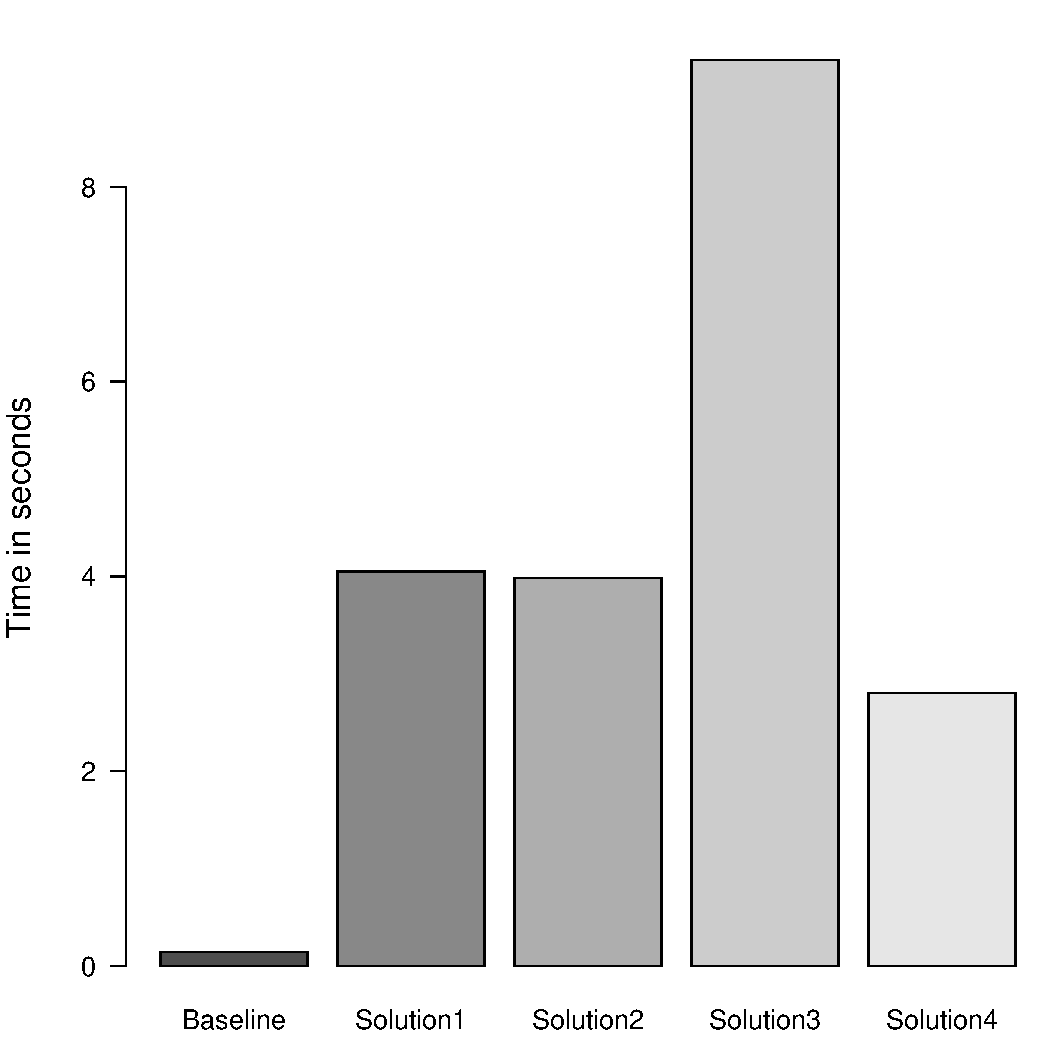
\includegraphics[width=\W]{figure/result/barplot-update_student-rt.pdf}}
			\subfigure[Update on Course]
			{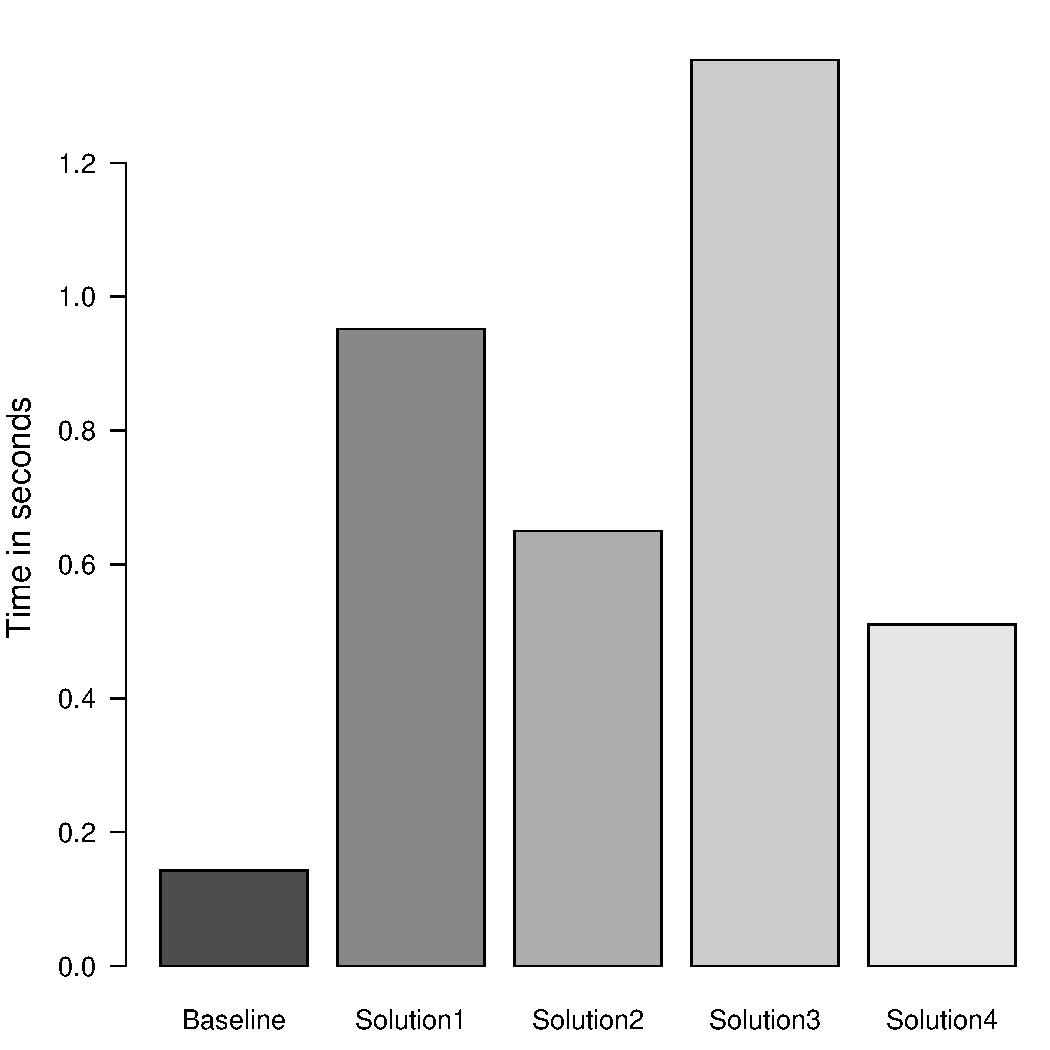
\includegraphics[width=\W]{figure/result/barplot-update_course-rt.pdf}}
			\subfigure[Update on Enrolment]
			{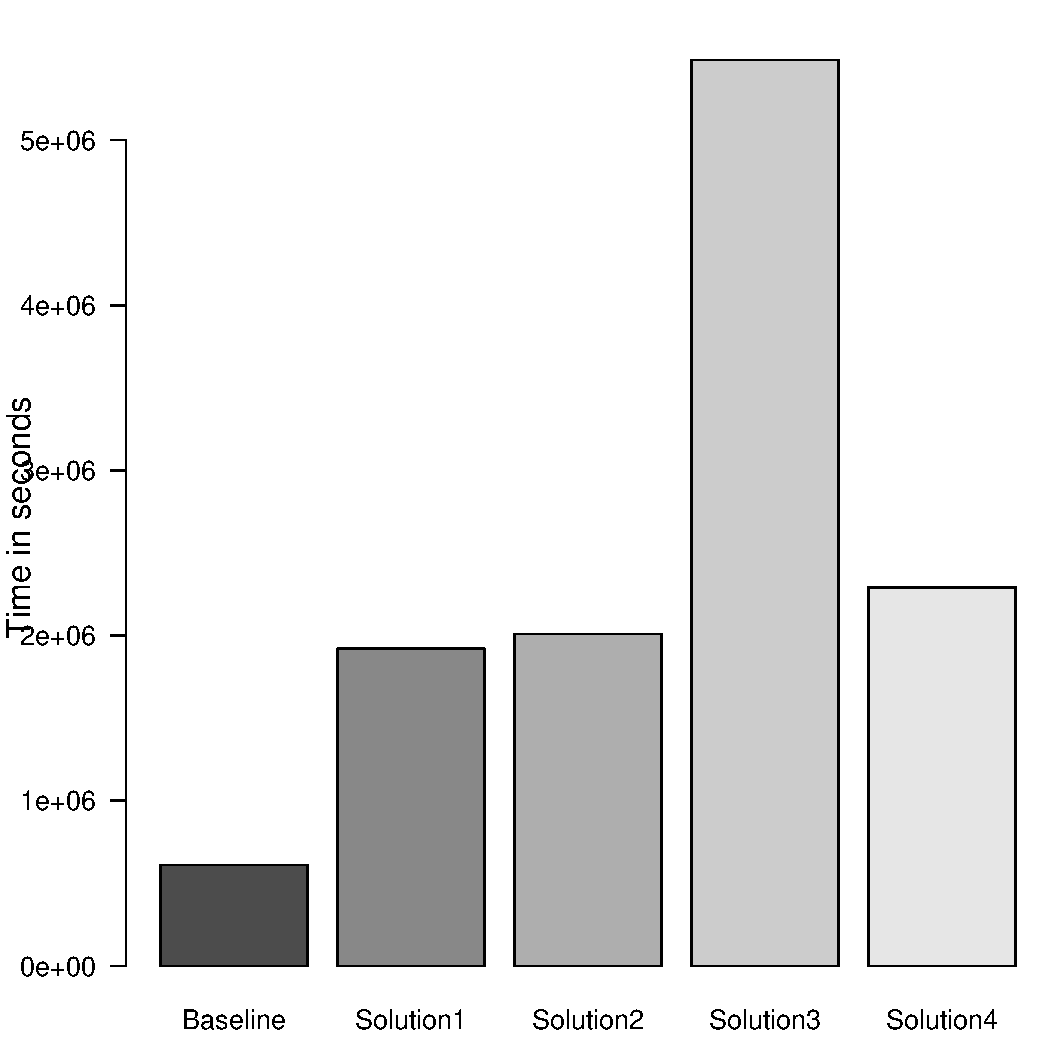
\includegraphics[width=\W]{figure/result/barplot-update_enrolment-rt.pdf}}
			\caption{Response time updating entities}\label{fres:update-response-time}
			
			\subfigure[Update on Student]
			{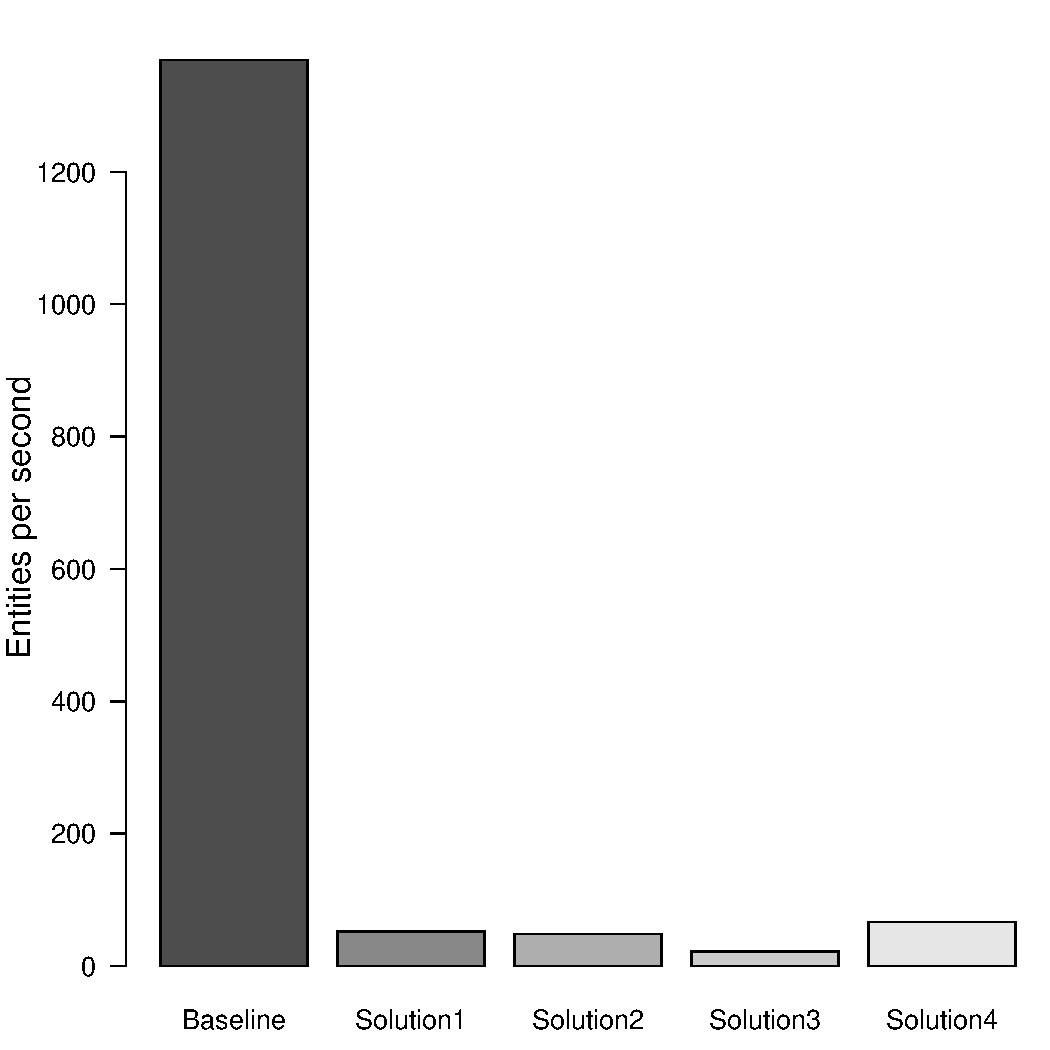
\includegraphics[width=\W]{figure/result/barplot-update_student-tp.pdf}}			
			\subfigure[Update on Course]
			{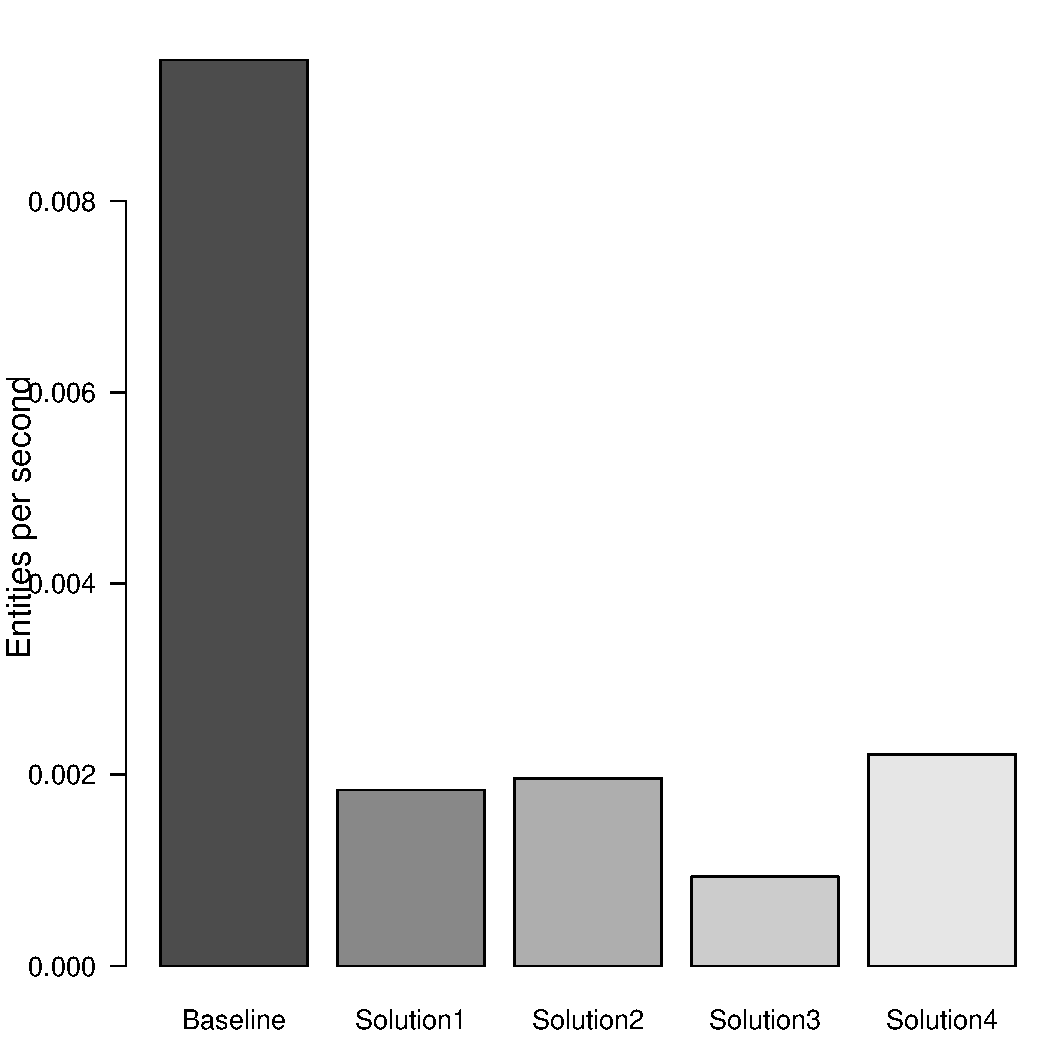
\includegraphics[width=\W]{figure/result/barplot-update_course-tp.pdf}}
			\subfigure[Update on Enrolment]
			{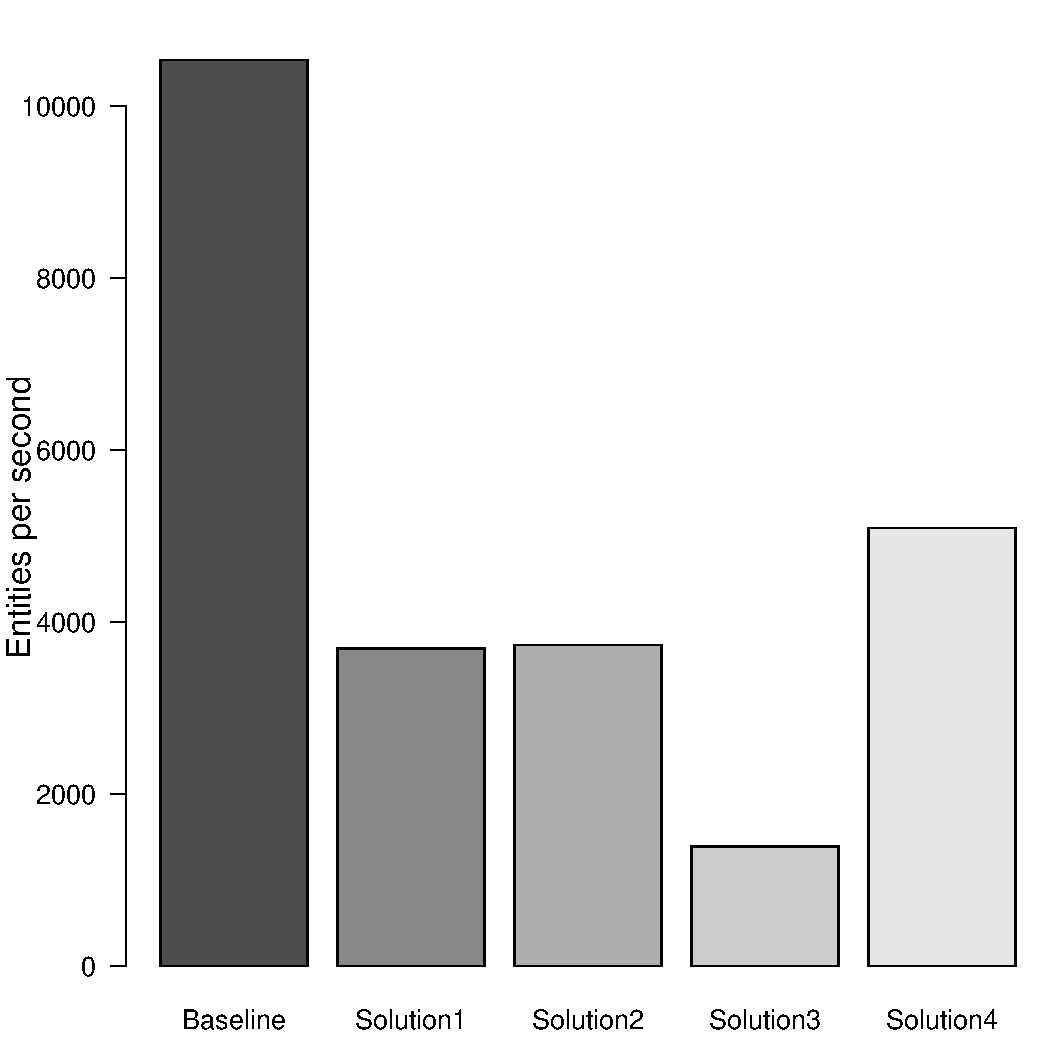
\includegraphics[width=\W]{figure/result/barplot-update_enrolment-tp.pdf}}
			\caption{Throughput updating entities}\label{fres:update-throughput}
		\end{figure}
 \end{landscape}